\documentclass[10pt]{beamer}

\newif\ifshowarchive
\showarchivetrue   % Change to \showarchivefalse to hide archived slides

\usetheme[progressbar=frametitle]{metropolis}
\usepackage{appendixnumberbeamer}

\usepackage{graphicx}
\usepackage{booktabs}
\usepackage{colortbl}
\usepackage[scale=2]{ccicons}

\usepackage{braket}
\usepackage{twemojis}

\usepackage{pgfplots}
\usepgfplotslibrary{dateplot}
\usepackage[font=scriptsize,labelfont=bf]{caption}

\usepackage{tikz}
\usetikzlibrary{fit,shapes,positioning,calc,shapes.geometric,backgrounds}
\colorlet{tempGray}{gray!80!cyan}
\colorlet{lightgray}{tempGray!60!white}
\colorlet{orange}{red!30!yellow}
\colorlet{lightorange}{orange!60!white}
\colorlet{darkGreen}{green!80!black}
\colorlet{paleGreen}{darkGreen!30!white}

\usepackage{xspace}
\newcommand{\themename}{\textbf{\textsc{metropolis}}\xspace}

\def\code#1{\texttt{#1}}
\newcommand{\lighthline}{\arrayrulecolor{gray!35}\hline\arrayrulecolor{black}}

\title{Quantum Technologies Research Project}
\subtitle{June Report}
\author{Linus Kelsey}
\date{24 Jun 26}
\institute{UCL Department of Physics and Astronomy \& \\ British Telecommunications}

\begin{document}
 
\maketitle

% GOALS ======================================================
\begin{frame}{Project Goals \& Metrics}
    \textbf{Research Gap:} No unified comparison of BB84 vs MDI-QKD across key metrics
    
    \begin{center}
        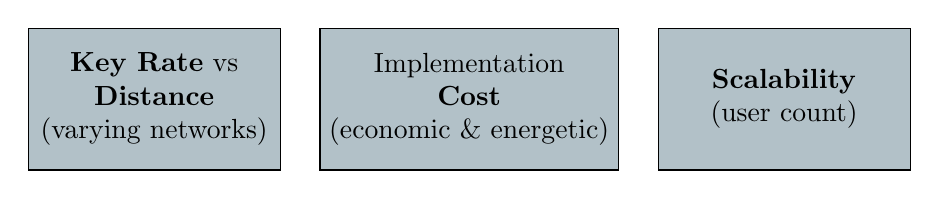
\begin{tikzpicture}
            \node[draw, fill=lightgray, minimum width=3.2cm, minimum height=1.8cm, align=center] at (0,0) {\textbf{Key Rate} vs\\\textbf{Distance}\\(varying networks)};
            \node[draw, fill=lightgray, minimum width=3cm, minimum height=1.8cm, align=center] at (4,0) {Implementation\\ \textbf{Cost}\\(economic \& energetic)};
            \node[draw, fill=lightgray, minimum width=3.2cm, minimum height=1.8cm, align=center] at (8,0) {\textbf{Scalability}\\(user count)};
        \end{tikzpicture}
    \end{center}
        
    \begin{itemize}
        \item Analyse both protocols across varying network topologies
        \item Identify parameter regimes \& topologies where each excels
        \item Inform practical QKD deployment decisions
    \end{itemize}
\end{frame}

% RECAP ======================================================
\begin{frame}{Where We Were}
    \begin{center}
    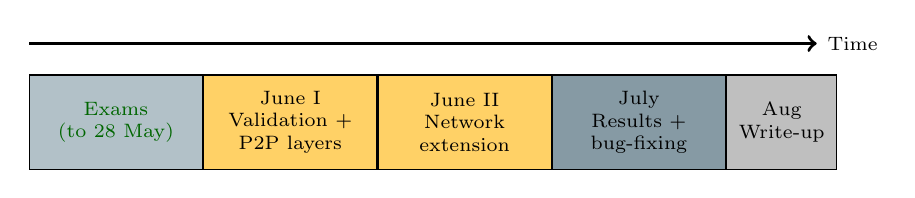
\begin{tikzpicture}[every node/.style={font=\scriptsize, align=center}]
        \draw[->, very thick] (0,1) -- (10,1) node[right] {Time};
 
        \node[draw, fill=lightgray, minimum width=2.2cm, minimum height=1.2cm, text=darkGreen!50!black] (exams) at (1.1, 0)
            {Exams\\(to 28 May)};
        \node[draw, fill=lightorange, minimum width=2.2cm, minimum height=1.2cm, right=0cm of exams] (june1) 
            {June I\\Validation +\\P2P layers};
        \node[draw, fill=lightorange, minimum width=2.2cm, minimum height=1.2cm, right=0cm of june1] (june2) 
            {June II\\Network\\extension};
        \node[draw, fill=tempGray, minimum width=2.2cm, minimum height=1.2cm, right=0cm of june2] (july) 
            {July\\Results +\\bug-fixing};
        \node[draw, fill=gray!50, minimum width=1.4cm, minimum height=1.2cm, right=0cm of july] 
            {Aug\\Write-up};
    \end{tikzpicture}
    \end{center}
    \vspace{0.1cm}
    \small
    \begin{itemize}
        \item \textbf{June first half:} \textcolor{orange!80!black}{Validation benchmarking} (BB84 + MDI); complete \textcolor{darkGreen!80!black}{P2P modelling} layers (dark counts $\to$ node loss $\to$ beyond)
        \item \textbf{June second half:} Begin \textcolor{darkGreen!80!black}{network-scale} extension; \textcolor{blue!80!black}{trusted node} \textcolor{darkGreen!80!black}{BB84 vs MDI} comparison
        \item \textbf{July:} \textcolor{darkGreen!80!black}{Bug-catching}, \textcolor{darkGreen!80!black}{parameter sweeps}, \textcolor{orange!80!black}{result collection}
        \item \textbf{August:} Write-up, final figures, submission preparation
        \item \textbf{September:} Viva
    \end{itemize}
\end{frame}

% PROGRESS ===================================================
\begin{frame}{Since last meeting}
    \textbf{May/June Progress}
    \begin{itemize}\small
        \item P2P modelling layers complete
        \item Network-level simulators built and tested
        \item Script suite with error analysis
        \item Hardware regime annotations
    \end{itemize}
    \vspace{0.2cm}
    \textbf{Action list}
    \begin{itemize}\small
        \item Effect of BB84 repeaters on comparison \hfill\twemoji{hourglass not done}
        \item Vary Charlie's location \hfill\twemoji{check mark button}
        \item Practical key rate thresholds (QBER $> 11\%$ cutoff) \hfill\twemoji{check mark button}
        \item One-pager: modelling plan \& layering \hfill\twemoji{hourglass done}
        \item Layered parameter analysis \hfill\twemoji{check mark button} 
    \end{itemize}
\end{frame}
 
% NETWORK ====================================================
\begin{frame}{Modelling Status: Network Modelling}
    \textbf{Metropolitan multi-user network model}
    \begin{itemize}\small
        \item $N$ randomly placed metropolitan users; \textbf{max connected logical layer}
        \item $K$ BSM nodes for MDI, all users fibre-connected for BB84
        \item Passive optical routing for cross-relay MDI pairs (as Q*Bird's)
    \end{itemize}
    \vspace{0.2cm}
    \textbf{Simulation experiments}
    \begin{itemize}\small
        \item \textbf{Exp 1 — relay sweep:} 
        \begin{itemize}
            \item fix $N$, vary $K$
            \item relay positions optimised by $k$-means
            \item identify optimal $K=K^*$
            \item compare with BB84 for given logical layer
            \item per-user pair Monte Carlo sims, as in P2P
        \end{itemize}
        \item \textbf{Exp 2 — user sweep:} fix $K=K^*$, vary $N$
    \end{itemize}
    \vspace{0.2cm}
    \textbf{Metrics:} average key rate; cost per unit key rate; keygen success rate
\end{frame}

% RESULTS I ==================================================
\begin{frame}{Results I: Further P2P Parameters}
    Swept \textbf{10 physical parameters}; realistic hardware regimes identified
    \vspace{0.1cm}
    \begin{center}
    \scriptsize
    \renewcommand{\arraystretch}{1.5}
    \begin{tabular}{ll}
        \toprule
        \textbf{Parameter(s)} & \textbf{Key finding} \\
        \midrule
        Fibre length \& loss & $\sim$Linear key rate drop-off for both protocols \\\lighthline
        Detector efficiency & MDI - quadratic decline; BB84 - linear \\\lighthline
        Dark counts, dephasing, source error & Negligible effect in investigated ranges \\\lighthline
        Node/connector loss \& basis bias & Linear declines; both steeper for MDI \\\lighthline
        Beam splitter efficiency & Shallow MDI decline within realistic range \\\lighthline
        Charlie placement & Peaks at midpoint; weak symmetric decay \\
        \bottomrule
    \end{tabular}
    \end{center}
\end{frame}

% RESULTS I ==================================================
\begin{frame}{Results I - cont.}
    \setlength{\fboxsep}{0pt}
    \vspace*{-0.2cm}
    \begin{center}
        \setlength{\tabcolsep}{0.4cm}
        \begin{tabular}{cc}
            \fbox{
\includegraphics[width=0.46\textwidth, height=3.5cm, keepaspectratio]{images/efficiency.png}} &
            \fbox{
\includegraphics[width=0.46\textwidth, height=3.5cm, keepaspectratio]{images/charlie_pos.png}} \\[0.4cm]
            \fbox{
\includegraphics[width=0.46\textwidth, height=3.5cm, keepaspectratio]{images/node_loss.png}} &
            \fbox{
\includegraphics[width=0.44\textwidth, height=3.5cm]{images/bs_eff.png}}
        \end{tabular}
    \end{center}
\end{frame}

% RESULTS II =================================================
\begin{frame}{Results II: Layered P2P Analysis}
    \vspace{0.42cm}
    Cumulative \textbf{layer build-up}, ideal $\to$ full physical model
    \setlength{\fboxsep}{0pt}
    \begin{center}
        \setlength{\tabcolsep}{0.2cm}
        \begin{tabular}{cc}
            \fbox{
\includegraphics[width=0.45\textwidth, height=5cm, keepaspectratio]{images/bb84_layers.png}} &
            \fbox{
\includegraphics[width=0.45\textwidth, height=5cm, keepaspectratio]{images/mdi_layers.png}}
        \end{tabular}
    \end{center}
    \textbf{Node loss} applies steepest drop from the prior layer for both. Other parameters cause marginal drops. Ideal conditions depart significantly from realistic.
\end{frame}

% RESULTS III ================================================
\begin{frame}{Results III: Early Network-Scale Results}
    \textbf{Exp 1 (relay sweep):} minimal rate penalty imposed by adding more BSM relays to MDI (example topology next slide). \textbf{Exp 2 (user sweep):} both protocols see shallow key rate decline when adding users.
    \setlength{\fboxsep}{0pt}
    \begin{center}
        \setlength{\tabcolsep}{0.2cm}
        \begin{tabular}{cc}
            \fbox{
\includegraphics[width=0.45\textwidth, height=5cm, keepaspectratio]{images/relay_count_20_users.png}} &
            \fbox{
\includegraphics[width=0.45\textwidth, height=4.65cm]{images/user_count.png}}
        \end{tabular}
    \end{center}
    BB84 outperforms MDI in network \textbf{more severely} than P2P link.
\end{frame}

% NETWORK VISUAL =============================================
\begin{frame}{Results III cont.}
    \setlength{\fboxsep}{0pt}
    \begin{center}
        \setlength{\tabcolsep}{0.2cm}
        \begin{tabular}{c}
            \fbox{
\includegraphics[width=\textwidth, keepaspectratio]{images/user_count_network_viz.png}}
        \end{tabular}
    \end{center}
    Relays placed by $k$-means clustering for MDI. \textbf{Multiple seeds} in single simulation produce distinct networks, rate curves average across these to \textbf{eliminate irregularities} in network generation.
\end{frame}
  
% NEXT =======================================================
\begin{frame}{Next Steps}
    \textbf{Simulation priorities:}
    \begin{itemize}
        \item Finalise hardware parameters from literature
        \item Overlay published BB84 + MDI curves/data points
        \item Data persistence for analysis
    \end{itemize}

    \vspace{0.15cm}
    \textbf{Analysis priorities:}
    \begin{itemize}
        \item Per-component hardware cost markers
        \item Identify regions where MDI/BB84 performance preferable
        \item Identify regimes where hardware is preferable
    \end{itemize}

    \textbf{Case Study} - microwave spin-ensemble realisation of quantum memories with Prof. John Morton (due 13 Jul 26)
\end{frame}

% TIMELINE ===================================================
\begin{frame}{Timeline}
    \begin{center}
    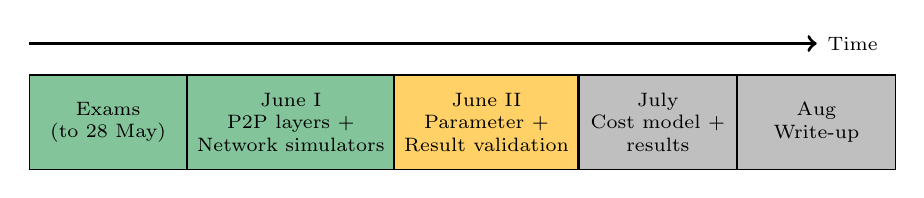
\begin{tikzpicture}[every node/.style={font=\scriptsize, align=center}]
        \draw[->, very thick] (0,1) -- (10,1) node[right] {Time};
 
        \node[draw, fill=darkGreen!20!lightgray, minimum width=2cm, minimum height=1.2cm] (exams) at (1, 0)
            {Exams\\(to 28 May)};
        \node[draw, fill=darkGreen!20!lightgray, minimum width=2.4cm, minimum height=1.2cm, right=0cm of exams] (june1) 
            {June I\\P2P layers +\\Network simulators};
        \node[draw, fill=lightorange, minimum width=2.2cm, minimum height=1.2cm, right=0cm of june1] (june2) 
            {June II\\Parameter +\\Result validation};
        \node[draw, fill=gray!50, minimum width=2cm, minimum height=1.2cm, right=0cm of june2] (july) 
            {July\\Cost model +\\results};
        \node[draw, fill=gray!50, minimum width=2cm, minimum height=1.2cm, right=0cm of july] 
            {Aug\\Write-up};
    \end{tikzpicture}
    \end{center}
    \vspace{0.1cm}
    \small
    \begin{itemize}
        \item \textbf{Remainder of June:} Hardware parameter range selection; literature result overlays; data storage
        \item \textbf{July:} cost model; result collection; Case Study; first draft; Singapore trip
        \item \textbf{August:} Write-up, final figures, submission preparation
        \item \textbf{September:} Viva
    \end{itemize}
\end{frame}

\end{document}
